\documentclass{beamer}
\usepackage{subfig}
\usetheme{Madrid}
\usepackage{chemfig}
\usepackage[version=4]{mhchem}
\title{Buffer solutions and application}
\author{Ahammad Musa \\ Roll: SH - 54 \\ Group: B - 08 \\ Session: 2014-15}
\institute{Department of Chemistry \\ University of Dhaka}
\date{July 18, 2017}
\begin{document}

\frame{\titlepage}

\begin{frame}
  \frametitle{Definition}
  A buffer solution is one which results change in pH when small quantities of acids or alkalies are added to it.
\end{frame}

\begin{frame}
  \frametitle{Type}
  There are two types of buffer solutions-
  \begin{itemize}
    \item Acidic buffer solution
    \item Alkaline buffer solution
  \end{itemize}
\end{frame}

\begin{frame}
  \frametitle{Type}
  \framesubtitle{Acidic buffer solution}
  Acidic buffer solutions are commonly prepared from a weak acid and its salt with a strong base.
 \begin{exampleblock}{Example}
    A mixture of \ce{CH3COOH} and \ce{CH3COONa} acts as an  acidic buffer.
 \end{exampleblock}
\end{frame}

\begin{frame}
  \frametitle{Type}
  \framesubtitle{Alkaline buffer solution}
  Alkaline buffer solution are commonly prepared from a weak base and its salt with a strong acid.
  \begin{exampleblock}{Example}
    A mixture fo \ce{NH4OH} and \ce{NH4Cl} acts as an alkaline buffer.
 \end{exampleblock}
\end{frame}

\begin{frame}
  \frametitle{Mechanism of Buffer Solution}
  \framesubtitle{Acidic buffer solution}
  To describe the mechanism fo acidic buffer solution we consider the acidic buffer solution prepared by \textbf{acetic acid} and \textbf{sodium acetate} as example.\\
    \ce{CH3COOH(aq) <=> CH3OO-(aq) + H+(aq)}
    \\
    \ce{CH3COONa(aq) -> CH3OO-(aq) + Na+(aq)}
\end{frame}

\begin{frame}
  \frametitle{Mechanism of Buffer Solution}
  \framesubtitle{Acidic buffer solution}
  \begin{description}[Removing of \ce{OH-} ion]
    \item[Removing of \chemfig{H^+} ion] When a small quantity of an acid is added the \chemfig{H^+} ions are removed by the reaction -
      \\
      \ce{H+(aq) + CH3COO-(aq) <=> CH3COOH(aq)}
    \item[Removing of \ce{OH-} ion] When a small quantity of base is added then the \ce{OH-} are neutralized by the reaction 
      \\
      \ce{OH-(aq) + H+(aq) -> H2O(l)}
  \end{description}
\end{frame}

\begin{frame}
  \frametitle{Mechanism of Buffer Solution}
  \framesubtitle{Alkaline buffer solution}
  To describe the mechanism of alkaline buffer solution we consider an alkaline buffer solution prepared by \textbf{ammonium hydroxide(\chemfig{NH_4OH})} and \textbf{ammonium chloride(\chemfig{NH_4Cl})} as example.
  \\
  \ce{NH4OH(aq) <=> NH4+(aq) + OH-(aq)} \\ 
  \ce{NH4Cl(aq) -> NH4+(aq) + Cl-(aq)}
\end{frame}

\begin{frame}
  \frametitle{Mechanism of Buffer Solution}
  \framesubtitle{Alkaline buffer solution}
  \begin{description}[Removing of \ce{OH-} ion]
    \item[Removing of \chemfig{H^+} ion] When a small quantity of strong acid is added to this solution the \chemfig{H^+} ions are removed as -
      \\
      \ce{H+(aq) + NH4OH(aq) -> NH4+(aq) + H2O(l)}
    \item[Removing of \ce{OH-} ion] When a small quantity of strong base is added to this solution the \ce{OH-} ions are removed as - 
      \\
      \ce{OH-(aq) + NH4+(aq) <=> NH4OH}
  \end{description}
\end{frame}

\begin{frame}
  \frametitle{pH calculation from solution}
  The pH of an acidic or basic buffer can be calculated by using Henderson-Hasselbalch equation.\\
  For acidic buffer solution-\\
    pH = pk\textsubscript{a} + \log{\tfrac{[salt]}{[acid]}}
    \\
    \newline
  For alkaline buffer solution-\\
    pH = pk\textsubscript{w} - pk\textsubscript{b} - \log{\tfrac{[salt]}{[base]}}
\end{frame}

\begin{frame}
  \frametitle{Buffer capacity}
  The buffer capacity of any buffer gives a measure of the amount of acid or alkali that the buffer can react with before changing the pH of the solution. The larger is the amounts of acid and its conjugate base or the base and its conjugate acid needed to change the pH of the buffer, the greater is the buffer capacity. Buffer capacity is high when, \tfrac{[salt]}{[acid]}=1.


\end{frame}

\begin{frame}
  \frametitle{Application}
  There are many applications of buffer solutions. Some are - 
  \begin{itemize}
    \item Many biological processes can only occur of very specific pH values. The reactions often take place in buffered environments. A buffer of \textbf{Carbonic acid(\ce{H2CO3})} and \textbf{bicarbonate(\ce{HCO3-})} is present in blood plasma, to maintain a pH between 7.35 and 7.45. Other fluids such as tear, salivary, urine, enzymes etc. has definite pH value. Eventhough the drugs that we take in our body has specific pH values.
    \item Industrially, buffer solutions are used in fermentation processes and in setting the correct conditions for dyes used in colouring fabrics. Also pH controlled in shampoo, soap, cosmetics etc.
  \end{itemize}
\end{frame}

\begin{frame}
  \frametitle{Application}

  \begin{figure}
    \subfloat[Blood]{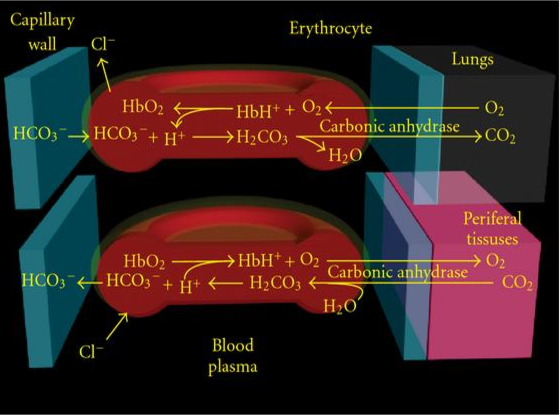
\includegraphics[width=5cm,height=5cm]{blood}} \qquad
    \subfloat[Dye]{\includegraphics[width=5cm,height=5cm]{pigments}}

  \end{figure}
\end{frame}

\begin{frame}
  \begin{center}
  \Huge{Thank You}
  \end{center}
\end{frame}

\end{document}
